\chapter{Introduction}
    Deep learning is an artificial intelligence function that imitates the workings of the human brain in processing data and creating patterns for use in decision making. Deep learning is a subset of machine learning in artificial intelligence (AI) that has networks capable of learning unsupervised from data that is unstructured or unlabeled. Also known as deep neural learning or deep neural network. Deep Learning is about learning multiple levels of representation and abstraction that help to make sense of data such as images, sound, and text.
\par
     In Artificial Intelligence (AI), we can think of machine learning (ML) as one of AI’s smaller subsets. Machine learning uses statistical techniques to provide computer systems ability to progressively improve its performance on a specific task with data without being explicitly programmed. Unsupervised learning algorithms are a subset of machine learning algorithms which tries to describe the structure of unlabelled data. Generative models is an approach to unsupervised learning. The goal of a generative model is to generate data similar to the ones in the dataset. Generative Adversarial Network (GAN) is a type of Generative Model. Other types of generative models include Variational Autoencoders (VAEs) and autoregressive models like PixelRNN. GANs have been successfully applied to solve problems in various domains like generating images, videos and audio, text to image synthesis etc. GANs were originally introduced by Ian Goodfellow and his collaborators in University of Montreal in 2014 . Yann LeCun, Director of AI Research at Facebook and Professor at NYU called adversarial training as "the most interesting idea in the last 10 years in ML" . 
\par
    
     Deep learning is a subset of machine learning in artificial intelligence (AI) that has networks capable of learning unsupervised from data that is unstructured or unlabeled. Also known as deep neural learning or deep neural network. The resolution and quality of images produced by generative methods especially generative adversarial networks (GAN) have seen rapid improvement recently. Yet the generators continue to operate as black boxes, and despite recent efforts, the understanding of various aspects of the image synthesis process, e.g., the origin of stochastic features, is still lacking. 
\par
    The properties of the latent space are also poorly understood, and the commonly demonstrated latent space interpolations provide no quantitative way to compare different generators against each other. Persuaded by style transfer literature, re-designing of the generator architecture in a way that exposes novel ways to control the image synthesis process. The modified generator architecture starts from a learned constant input and adjusts the “style” of the image at each convolution layer based on the latent code, therefore directly controlling the strength of image features at different scales. Combining the gaussian noise  injected directly into the network, this architectural change leads to automatic, unsupervised separation of high-level attributes (e.g., pose, identity) from stochastic variation (e.g., freckles, hair) in the generated images, and enables intuitive scale-specific mixing. The discriminator and the loss functions are not altered in the new architecture so that it  was orthogonal to the GAN loss functions, regularization, and hyperparameters. The result of the style based GAN was a new dataset of human faces (Flickr-Faces-HQ, FFHQ) . The FFHQ database contains the images with 1024 * 1024 resolution, which is much better than the benchmark image resolutions used for the industrial problems. 



\section{The Perceptron}
    The Perceptron is one of the simplest ANN architectures, invented in 1957 by Frank Rosenblatt. It is based on a slightly different artificial neuron called a linear threshold unit (LTU): the inputs and output are now numbers (instead of binary on/off values) and each input connection is associated with a weight. The LTU computes a weighted sum of its inputs (z = w1 x1 + w2 x2 + ... + wn xn = wT · x), then applies a step function to that sum and outputs the result. LTU is only a concept, by applying a learning rule to the LTU results in the percepton. The problem with the perceptron is that its only possible for binary classification problems.
    
    \begin{figure}[h]
        \centering
        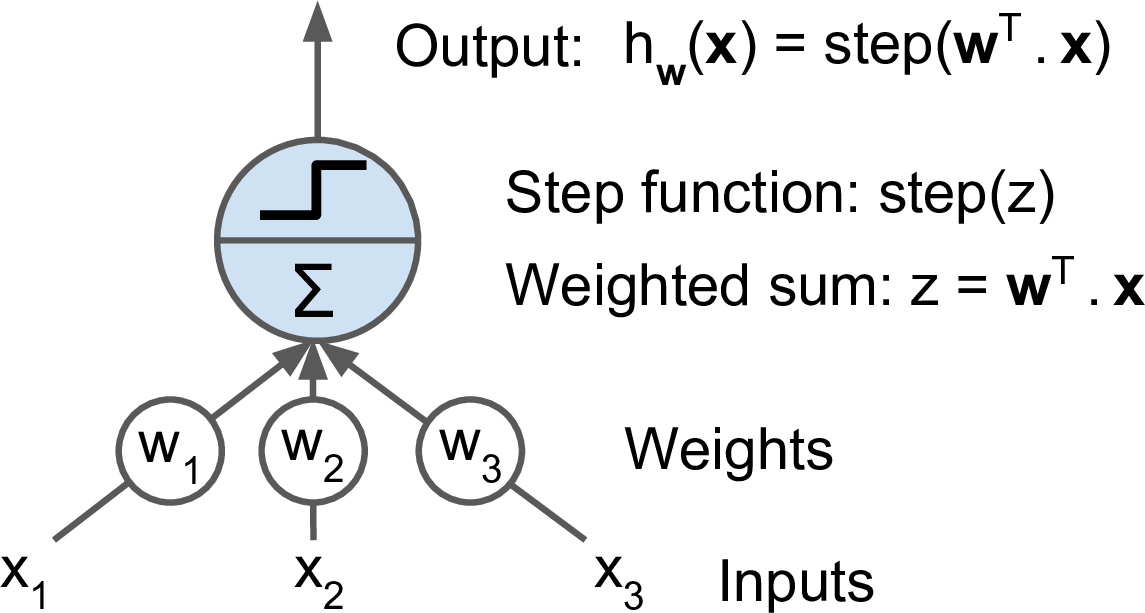
\includegraphics[width=0.5\linewidth]{perceptron.png}
        \caption{Perceptron}
        \label{fig:perceptron}
    \end{figure} 
\section{Multi-Layer Perceptron and Backpropagation}
    An MLP is composed of one (passthrough) input layer, one layers of LTUs, called hidden layers, and one final layer of LTUs called the output layer. Every layer except the output layer includes a bias neuron and is fully connected to the next layer.  To create a multi layer perceptron, multiple LTUs are stacked side by side and on the top. As this was mainly used for multi class classification problem, the activation function used will be sigmoid activation.
    \begin{figure}[h]
        \centering
        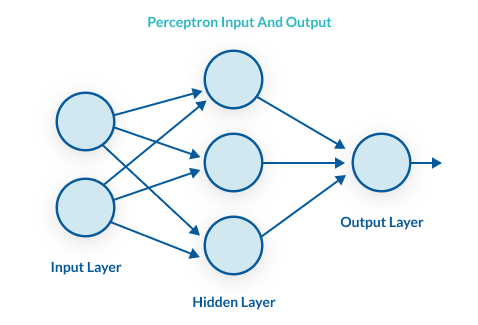
\includegraphics[width=0.5\linewidth]{mlp.png}
        \caption{Multi Layer Perceptron}
        \label{fig:perceptron}
    \end{figure} 
\section{Deep Neural Network}
    If only single hidden layer was used in an architecture it is known as MLP.  If multiple hidden layers are used in the architecture it is known as deep neural networks. A learning weights in a deep neural network is known as Deep Learning.
    \begin{figure}[h]
        \centering
        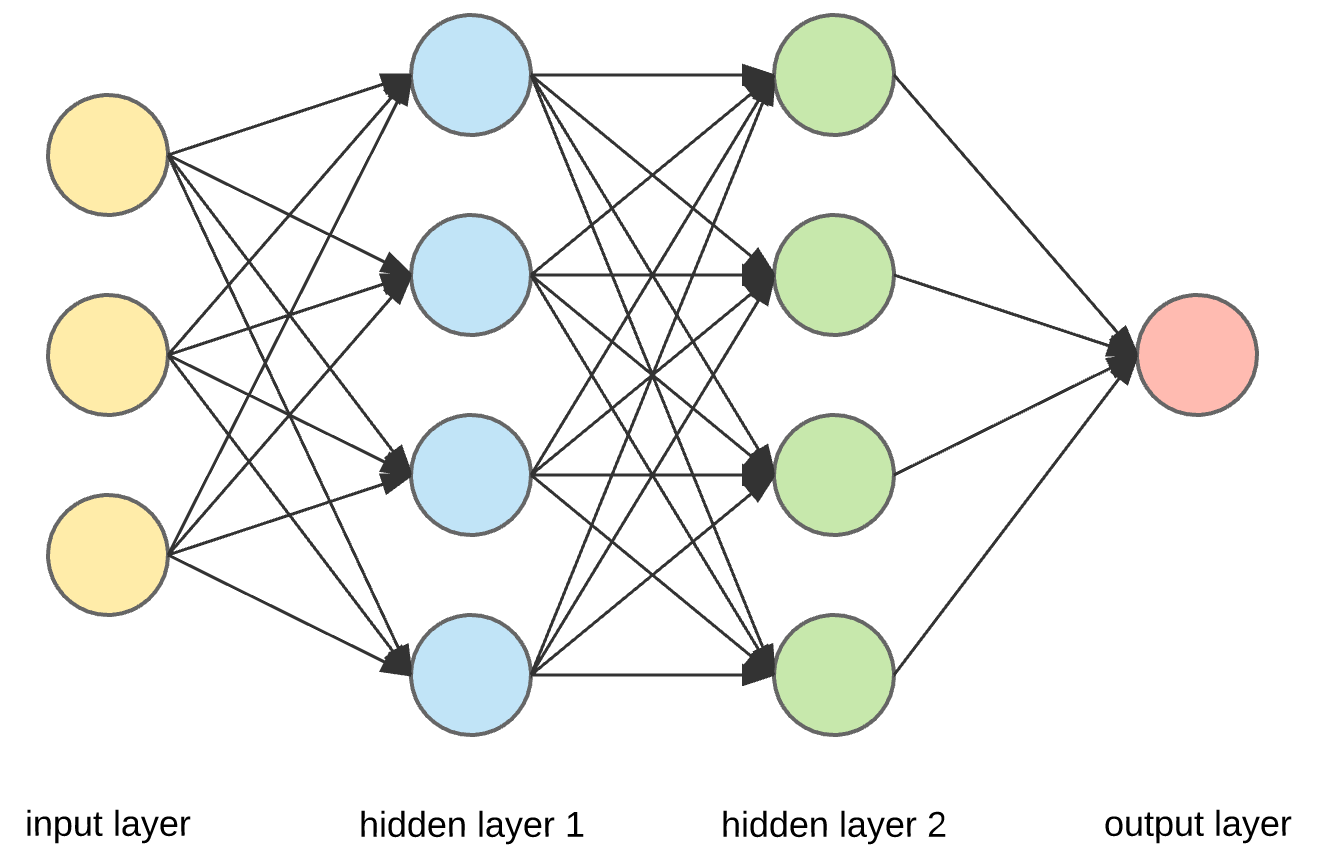
\includegraphics[width=0.5\linewidth]{dnn.png}
        \caption{Deep Neural Network}
        \label{fig:perceptron}
    \end{figure} 
\section{Convolutional Neural Networks}
    While dealing with image data, deep neural networks fails upto an extend as it cant extract the structural information from the images.  CNN image classifications takes an input image, process it and classify it under certain categories. Computers sees an input image as array of pixels and it depends on the image resolution. Based on the image resolution, it will see h x w x d( h = Height, w = Width, d = Dimension ). Eg., An image of 6 x 6 x 3 array of matrix of RGB (3 refers to RGB values) 
    \begin{figure}[h]
        \centering
        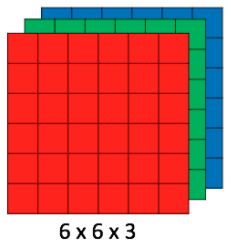
\includegraphics[width=0.2\linewidth]{matrix.png}
        \caption{Array representation of an image}
        \label{fig:Array representation of an image}
    \end{figure} 
    
    Technically, deep learning CNN models to train and test, each input image will pass it through a series of convolution layers with filters (Kernals), Pooling, fully connected layers (FC) and apply Softmax function to classify an object with probabilistic values between 0 and 1. 
    Convolution is the first layer to extract features from an input image. Convolution preserves the relationship between pixels by learning image features using small squares of input data. It is a mathematical operation that takes two inputs such as image matrix and a filter or kernal. Convolution of an image with different filters can perform operations such as edge detection, blur and sharpen by applying filters.(Kernels). Stride is the number of pixels shifts over the input matrix. When the stride is 1 then we move the filters to 1 pixel at a time.Sometimes filter does not fit perfectly fit the input image. We have two options:
        \begin{itemize}
            \item Pad the picture with zeros (zero-padding) so that it fits.
            \item Drop the part of the image where the filter did not fit. This is called valid padding which keeps only valid part of the image.
        \end{itemize}
     Pooling layers section would reduce the number of parameters when the images are too large. Spatial pooling also called subsampling or downsampling which reduces the dimensionality of each map but retains the important information. Spatial pooling can be of different types:
        \begin{itemize}
            \item Max Pooling
            \item Average Pooling
            \item Min pooling
        \end{itemize}

    In the layer we call as FC layer, we flattened our matrix into vector and feed it into a fully connected layer like Deep neural network.
    \begin{figure}[h]
        \centering
        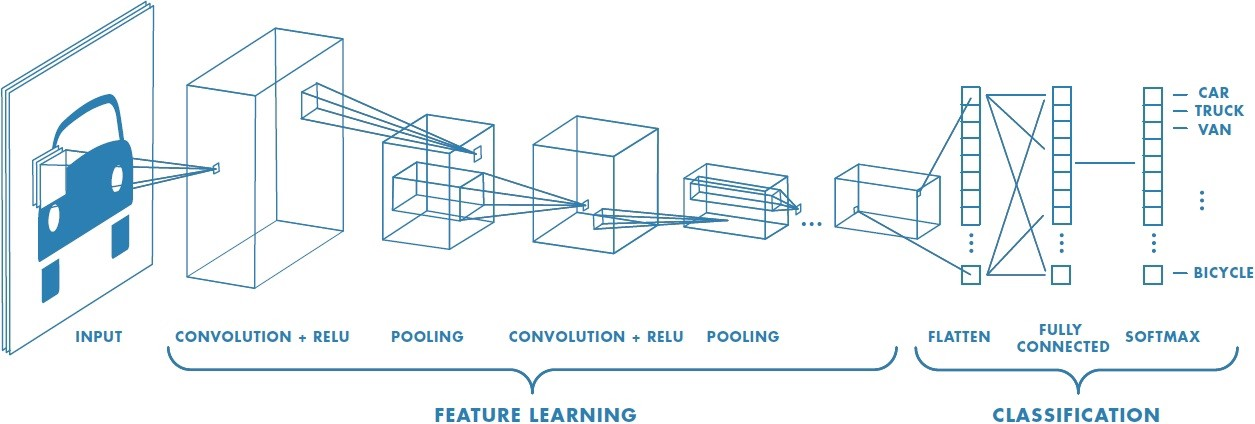
\includegraphics[width=0.5\linewidth]{cnn.png}
        \caption{Convolutional Neural Network model}
        \label{fig:Convolutional Neural Network model}
    \end{figure} 
